\documentclass[fleqn,11pt,openany]{book}

% These two need to be set before including scirun style package
\title{SCIRun Module Generation}
\author{Jess Tate}

% INCLUDE SCI STYLE DOCUMENT
\usepackage{scirun}

\begin{document}

%% starting from SCIRun Doc wiki
%% http://software.sci.utah.edu/SCIRunDocs/index.php/CIBC:Documentation:SCIRun:Tutorial:BioPSE


% CREATE TITLE PAGE --------------------------------------------------
\maketitle

% CHAPTERS ---------------------------------------------------------------

\chapter{SCIRun Overview} \label{overview}

\begin{introduction}
This tutorial demonstrates how to create new modules in SCIRun \SCIRunVersion.  It will walk through all the files needed and the basic module structure used by modules.  These instructions assume a basic understanding in C++ coding and other basic programing skills
\end{introduction}

\section{Software requirements}

\subsection{SCIRun  \SCIRunVersion}

Download SCIRun version \SCIRunVersion  from the \href{http://www.scirun.org}{SCI software portal}.
Make sure to update to the most up-to-date version of the source code available, which will include the latest bug fixes.
Alternatively, use git to clone the SCIRun repository (https://github.com/SCIInstitute/SCIRun.git).  
We suggest creating a fork of the repository so that you can track your changes and create pull requests to the SCIRun repository (Section \ref{sec:forking}).  
%See github and git documentation on how to create, sync, merge, and manage forks

\subsection{Compilers, Dependencies Development Tools}

SCIRun will need to be built from the source code in order to test and use any modules written.  
Make sure that qt 4.8, git, cmake, and the latest c++ compilers for the operating system are installed.  

\subsection{Creating Your SCIRun Fork}
\label{sec:forking}

With your own github account, go to the \href{https://github.com/SCIInstitute/SCIRun}{SCIRun github page}.
Click the fork button on the upper right side of the page.  
It will ask you where to move the fork to, chose your own account.  
Once the repository is forked, clone it to your local machine with the following command.  
\begin{verbatim}
$ git clone https://github.com/[yourgithubaccount]/SCIRun.git
\end{verbatim}
After the the code is cloned, navigate to the repository directory and add the upstream path to the original SCIRun repository.
\begin{verbatim}
$ git remote add upstream https://github.com/SCIInstitute/SCIRun.git
\end{verbatim}
You should be able to see both your and the original repositories when you use the command:
\begin{verbatim}
$ git remote -v
\end{verbatim}
The fork is good to go, but you will need to sync the fork occationally to keep up with the changes in the main repository.  To sync your fork, use the following commands:
\begin{verbatim}
$ git fetch upstream
$ git checkout master
$ git merge upstream/master
\end{verbatim}
You should sync and merge your fork before you start a new module and before you create a pull request.  
It is a good practice to create a new branch in your fork for every module you will be adding.  The command to create a new branch is:
\begin{verbatim}
$ git checkout -b [branch_name]
\end{verbatim}
Please see the \href{https://help.github.com}{github help page} for more information.

\chapter{Files Needed for a New Module}
\label{sec:files}

\begin{introduction}
This chapter will describe the files need to create a module in SCIRun.

Scope: \hyperref[sec:overview]{Overview of Files Needed for each Module} - \hyperref[sec:config]{Module Configuration File} -
\hyperref[sec:module]{Module Source Code} - \hyperref[sec:algo]{Algorithm Code} - \hyperref[sec:ui]{Module UI Code}
\end{introduction}

\section{Overview of Files Needed for each Module}
\label{sec:overview}

There are only three files required to create a module, though more may be needed depending on the function of the module.
In addition to the required module source code and header files (\emph{modulename.cc} and \emph{modulename.h}), a module configuration file is needed.
The module configuration file (\emph{modulename.module}) contains a description of the module and its state and names all the files needed for the module to be included in SCIRUn.  

Simple modules without user interfaces (UIs) can be created with the previously list three files alone.
However, if the module function needs a UI, there are three additional files needed.  
SCIRun can generate a UI for a module without these, but the functionality will be very limited to nonexistent.  
The qt ui file (\emph{modulenameDialog.ui}) describes the graphics and hooks of the UI can be created using the qt UI editor.
Module UIs also require a code and header file (\emph{modulenameDialog.cc} and \emph{modulenameDialog.h}.

Most modules, especially those requiring more than minimal code, should also have algorithm code to allow for greater portability and code control.  
This algorithm code and header file (\emph{modulenameAlgo.cc} and \emph{modulenameAlgo.h}) should contain all the computation of the module.
Though it is possible to build modules without these algorithm files, it is considered good practice to do so.

It is worth noting that each of the \emph{CMakeLists.txt} files in the directories of all of the files (except the module config file).  
See the examples in the following chapters for details.  %TODO reference other chapters.


\section{Module Configuration File}
\label{sec:config}

The module configuration file contains all the information need for the module factory to create necessary linkage and helper files for module to be properly included into SCIRun.  
Module configuration files should be located in \emph{src/Modules/Factory/Config/}.  
It is a text file that describes fields specific to the module delimited by curly brackets.  
There are three fields ``module", ``algorithm", and ``UI" and within each field are subfields ``name" and ``header", and others depending on the field.  
The following is an example that reflects the template files included in the source code.
\begin{verbatim}
{
  "module": {
    "name": "@ModuleName@",
    "namespace": "Fields",
    "status": "description of status",
    "description": "description of module",
    "header": "Modules/Template/ModuleTemplate.h"
  },
  "algorithm": {
    "name": "@AlgorithmName@Algo",
    "namespace": "Fields",
    "header": "Core/Algorithms/Template/AlgorithmTemplate.h"
  },
  "UI": {
    "name": "@ModuleName@Dialog",
    "header": "Interface/Modules/Template/ModuleDialog.h"
  }
}
\end{verbatim}
This config file example would not build.  
We will include specific examples that will build and work in following chapters of this tutorial (Chapters---). %TODO reference other chapters.

As mentioned before, the UI and algorithm files are not required to generated a module, therefore the subfields for the ``algorithm" or ``UI" fields can changed to ``N/A" to indicate that these files do not exist.  
Please refer to Section~\ref{} for an example.  %TODO reference other chapters.

\section{Module Source Code}
\label{sec:module}

The Module source code consist of a .cc and .h file that code the actual function of the module.
However, since most modules use an algorithm file, these files can also be considered the the code that pulls all the relevant information from the algorithm, the UI, and other modules in order to achieve it's proper function.  
These files should be located in the proper directory with the \emph{src/Modules/} directory.
For example purposes, we will show and discuss the template files included in the \emph{src/Modules/Template/} directory.

\subsection{Module Header File}

The module header file functions as a typical C++ header file, containing code establishing the module object and structure.  
The \emph{ModuleTemplate.h} file found in \emph{src/Modules/Template/} provides an example of the kind of coding needed for a module header.  
The relevant functions are included here, with annotated comments:
\begin{verbatim}
// makes sure that headers aren't loaded multiple times. 
// This requires the string to be unique to this file.
// standard convention incorporates the file path and filename.
#ifndef MODULES_FIELDS_@ModuleName@_H__
#define MODULES_FIELDS_@ModuleName@_H__

#include <Dataflow/Network/Module.h>
#include <Modules/Fields/share.h>
// share.h must be the last include, or it will not build on windows systems.

namespace SCIRun {
namespace Modules {
namespace Fields {
// this final namespace needs to match the .module file
// in src/Modules/Factory/Config/
  
  // define module ports.  
  // Can have any number of ports (including none), and dynamic ports.
  class SCISHARE @ModuleName@ : public SCIRun::Dataflow::Networks::Module,
    public Has1InputPort<FieldPortTag>,
    public Has1OutputPort<FieldPortTag>
  {
  public:
    // these functions are required for all modules
    @ModuleName@();
    virtual void execute();
    virtual void setStateDefaults();
    
    //name the ports and datatype.
    INPUT_PORT(0, InputField, Field);
    OUTPUT_PORT(0, OutputField, Field);
  
    // this is needed for the module factory
    static const Dataflow::Networks::ModuleLookupInfo staticInfo_;
  };
}}}
#endif
\end{verbatim}
One of the key functions of this header file is the definition of the ports used by the module.  
This template uses one input and output, but any number can be used by changing the number and defining all the port types.
To use two inputs and outputs:
\begin{verbatim}
public Has2InputPorts<FieldPortTag,FieldPortTag>,
public Has2OutputPorts<FieldPortTag,FieldPortTag>
\end{verbatim}
If no there are no input or output ports, the commands are:
\begin{verbatim}
public HasNoInputPorts,
public HasNoOutputPorts
\end{verbatim}
Dynamic ports are also possible for the inputs.  
Dynamic ports are essentially a vector of ports, and are counted as a single port in the header.
For a single dynamic port, then a static port and a dynamic port:
\begin{verbatim}
public Has1InputPort<DynamicPortTag<FieldPortTag>>,
public Has2InputPorts<FieldPortTag,DynamicPortTag<FieldPortTag>>
\end{verbatim}






List of port tags that can be used in SCIRun:
\begin{itemize}
\item MatrixPortTag 
\item ScalarPortTag
\item StringPortTag
\item FieldPortTag
\item GeometryPortTag
\item ColorMapPortTag
\item BundlePortTag
\item NrrdPortTag
\item DatatypePortTag
\end{itemize}

\subsection{Module Code File}

\begin{verbatim}
#include <Modules/Fields/@ModuleName@.h>
#include <Core/Datatypes/Legacy/Field/Field.h>
#include <Core/Algorithms/Field/@ModuleName@Algo.h>

using namespace SCIRun::Modules::Fields;
using namespace SCIRun::Core::Datatypes;
using namespace SCIRun::Dataflow::Networks;
using namespace SCIRun::Core::Algorithms::Fields;

// this defines the location of the module in the module list.  
// "NewField" is the catagory and "SCIRun" is the package.
const ModuleLookupInfo @ModuleName@::staticInfo_("@ModuleName@", 
          "NewField", "SCIRun");

@ModuleName@::@ModuleName@() : Module(staticInfo_)
{
  //initialize all ports.
  INITIALIZE_PORT(InputField);
  INITIALIZE_PORT(OutputField);
}

void @ModuleName@::setStateDefaults()
{
  auto state = get_state();
  setStateBoolFromAlgo(Parameters::Knob1);
  setStateDoubleFromAlgo(Parameters::Knob2);
}

void @ModuleName@::execute()
{
  // get input from ports
  auto field = getRequiredInput(InputField);
  // get parameters from UI
  setAlgoBoolFromState(Parameters::Knob1);
  setAlgoDoubleFromState(Parameters::Knob2);
  // run algorithm code.  
  auto output = algo().run(withInputData((InputField, field)));
  //send to output port
  sendOutputFromAlgorithm(OutputField, output);
}
\end{verbatim}


\section{Algorithm Code}
\label{sec:algo}


\section{Module UI Code}
\label{sec:ui}


\subsection{Module Design File}

\begin{figure}[H]
\scalebox{0.3}{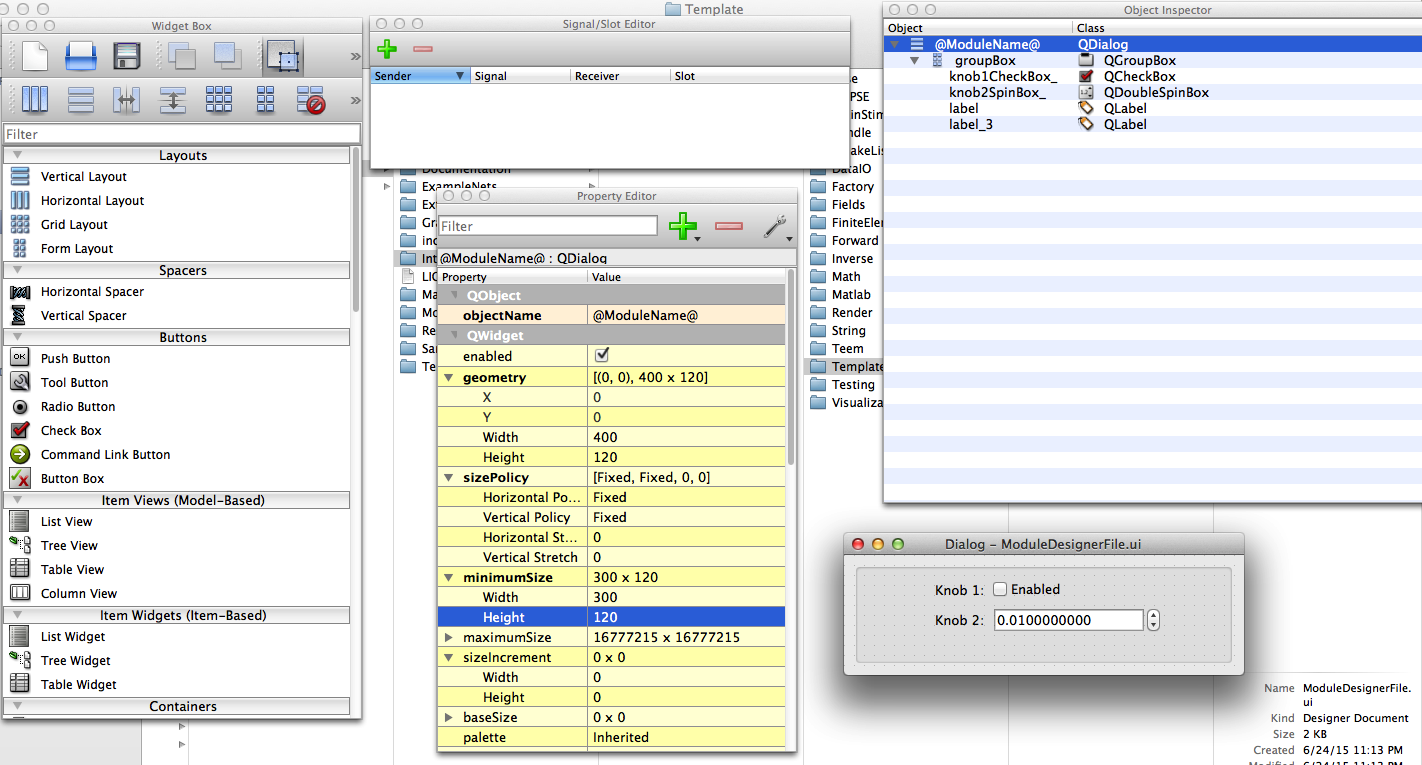
\includegraphics{SCIRun5ModuleGeneration_Figures/QT-editor.png}}
\caption{Template module interface design file as seen in the Qt editor.}
\label{fig:qteditor}
\end{figure}


%%%%%%%%%%%%%%%%%%%%%%%%%%%%%%%%%%%

\chapter{Example: Simple Module Without UI}

\begin{introduction}
This chapter describes how to create a very simple module in SCIRun.  
We will show how to make a simple module that outputs a simple string.  
This example will show the basics of the functions and code used by SCIRun to create and run modules.

Scope: \hyperref[sec:examp_config]{Module Config File} - \hyperref[sec:examp_header]{Module Header File} - \hyperref[sec:examp_source]{Module Source Code} - \hyperref[sec:testing]{Building and Testing}
\end{introduction}

\section{Module Config File}
\label{sec:examp_config}

If you have created a fork from the SCIRun git repository, begin by creating a new branch in your repository.  
Be sure to commit your changes to your repository often, as this can help you and the developers fix and make improvements to the code.
It is often easiest to modify existing code to fit your purposes than create new code, so determine a module that has similar functionality or structure to the new module.  
If desired, there is also the template files described in Chapter~\ref{sec:files} to use as a basis.  
In this example, we will provide the code needed, so it is not necessary to copy another module.  

%TODO maybe make a branch with examples?

Begin with the module config file.  
Create a new text file in module factory configuration directory (\emph{src/Modules/Factory/Config/}) for the new module.  
I should be named \emph{TestModuleSimple.module} or something similar.  
The text of the file should be:
\begin{verbatim}
{
  "module": {
    "name": "TestModuleSimple",
    "namespace": "StringManip",
    "status": "new module",
    "description": "This is a simple module to show how to make new modules.",
    "header": "Modules/String/TestModuleSimple.h"
  },
  "algorithm": {
    "name": "N/A",
    "namespace": "N/A",
    "header": "N/A"
  },
  "UI": {
    "name": "N/A",
    "header": "N/A"
  }
}
\end{verbatim}
The exact text of the status and description can be whatever the creator desires. 
The names of the module and filenames can also be different, but they must match the module code.  

\section{Module Header File}
\label{sec:examp_header}

Now we move to the module code.
The module will need to be placed in one of the directories in \emph{src/Modules/}, so choose the directory that fits the modules use the best (do not place the module code in \emph{Factory} or \emph{Template}, and \emph{Legacy} is generally for converted modules from earlier versions of SCIRun)
Since this module will be only have a string output, we will place the module code in \emph{src/Modules/String/}.
In this directory create a file called \emph{TestModuleSimple.h}.  
This file will be very similar to the \emph{ModuleTemplate.h} file shown earlier.
In addition to the SCIRun license information, the content of the header file should be:
\begin{verbatim}
#ifndef MODULES_STRING_TestModuleSimple_H
#define MODULES_STRING_TestModuleSimple_H

#include <Dataflow/Network/Module.h>
#include <Modules/Fields/share.h>

namespace SCIRun {
namespace Modules {
namespace StringManip {

class SCISHARE TestModuleSimple : public SCIRun::Dataflow::Networks::Module,
public HasNoInputPorts,
public Has1OutputPort<StringPortTag>
{
public:
  TestModuleSimple();
  virtual void execute();
  virtual void setStateDefaults() {};
  
  OUTPUT_PORT(0, OutputString, String);
  
  static const Dataflow::Networks::ModuleLookupInfo staticInfo_;
};
}}}
#endif
\end{verbatim}
As mentioned in Section~\ref{sec:config}, the header files for most modules do not vary significantly.  
This example in particular contains only elements common to most other modules.
The key to creating the header files is to ensure that the module name is correct in every place it occurs, that the namespace (StringManip) matches the module config file and that the ports are numbered and labeled correctly.  

\section{Module Source Code}
\label{examp_source}

The final file needed for this module is the source code file (\emph{ModuleTemplate.cc}).
The functionality used in this module is minimal to show how the essential functions.  
With the license and other comments, the file should contain:
\begin{verbatim}
#include <Modules/String/TestModuleSimple.h>
#include <Core/Datatypes/String.h>

using namespace SCIRun;
using namespace SCIRun::Modules::StringManip;
using namespace SCIRun::Core::Datatypes;
using namespace SCIRun::Dataflow::Networks;

/// @class TestModuleSimple
/// @brief This module splits out a string. 

const ModuleLookupInfo TestModuleSimple::staticInfo_("TestModuleSimple", 
       "String", "SCIRun");

TestModuleSimple::TestModuleSimple() : Module(staticInfo_,false)
{
  INITIALIZE_PORT(OutputString);
}

void
TestModuleSimple::execute()
{  
  std::string message_string;
  
  message_string = "[Personalize your  message here.]";
  
  StringHandle msH(new String(message_string));
  sendOutput(OutputString, msH);
}
\end{verbatim}

\section{Building and Testing}
\label{sec:testing}

After these files are modified correctly,  the only step remaining before building is adding the module code and header to the compiler list.  
Open the \emph{src/Modules/String/CMakeLists.txt} file.  
Add \emph{TestModuleSimple.cc} and \emph{TestModuleSimple.h} to the respective list.
There will more to the file, but the relevant sections should look something like this:
\begin{verbatim}
SET(Modules_String_SRCS
  CreateString.cc
  NetworkNotes.cc
  TestModuleSimple.cc
)

SET(Modules_String_HEADERS
  CreateString.h
  NetworkNotes.h
  share.h
  TestModuleSimple.h
)
\end{verbatim}

After changing the CMakeList.txt file, build SCIRun using the build script, or if you have already built SCIRun recently, go to the \emph{SCIRun\_root/bin/SCIRun} directory and run make.  
Take note of any build errors, if there is a problem in the with any module factory files, make sure that there are no mistakes in the the module configuration file and build again.  
Check out the common build errors in section [TODO]. %TODO, add section reference

After SCIRun builds completely, Launch SCIRun and test the module.  
You can use the PrintDatatype module to view the string that this module outputs. 
Other modules will require more testing, but due to the very simple nature of the module you can know that if the messages matches what you expect, then it is working properly.  

%%%%%%%%%%%%%%%%%%%%%%%%%%%%%%%%%%%%%%%%%%%%%%%%%%%%%%%%%%%

\chapter{Example: Simple Module With UI}

\begin{introduction}
In this chapter, we will build off the module that we described in the previous chapter to show how to add a UI and an input port.  
This module will print a message that comes from either the input port or the UI.  
We will show how to add a UI incrementally to help convey the principles that the software is based upon.
This incremental approach allows the user to copy this approach with more complicated module as it provides sanity checks for the user.

Scope: \hyperref[sec:duplicate]{Duplicate the Previous Module} - \hyperref[sec:addUI]{Creating a Custom UI} -
\hyperref[connectUI]{Connecting UI to the Module} - \hyperref[sec:addinput]{Adding an Input Port} - \hyperref[sec:finished]{Finished Code}
\end{introduction}

\section{Duplicate the Previous Module}
\label{sec:duplicate}

To begin, copy the \emph{TestModuleSimple.module} in the \emph{src/Modules/Factory/Config/} and name the copy \emph{TestModuleSimpleUI.module}.
Change the name and header field to reflect the new name of the module, as shown here:
\begin{verbatim}
  "module": {
    "name": "TestModuleSimpleUI",
    "namespace": "StringManip",
    "status": "new module",
    "description": "This is a simple module to show how to make new modules.",
    "header": "Modules/String/TestModuleSimpleUI.h"
  },
\end{verbatim}
For now, leave the rest of the fields as 'N/A'; we will come back to those.  

Next, copy the module code files \emph{TestModuleSimple.h} and \emph{TestModuleSimple.cc} in the \emph{src/Modules/String/} directory and rename them appropriately (\emph{TestModuleSimpleUI.h} and \emph{TestModuleSimpleUI.cc}).  
In these new files, change all the references of the modules name to TestModuleSimpleUI. 
A find and replace function will manage most instances, but make sure that all of them are changed. 
There are 4 lines in each of the two files that need to be changed, with more than one change in some lines.
The changes in \emph{TestModuleSimpleUI.h} are these lines:
\begin{verbatim}
#ifndef MODULES_STRING_TestModuleSimpleUI_H
#define MODULES_STRING_TestModuleSimpleUI_H

...

class SCISHARE TestModuleSimpleUI : public SCIRun::Dataflow::Networks::Module,

...

public:
  TestModuleSimpleUI();

...  

\end{verbatim}
And for the \emph{TestModuleSimpleUI.cc} file:
\begin{verbatim}
#include <Modules/String/TestModuleSimpleUI.h>

�

const ModuleLookupInfo TestModuleSimpleUI::staticInfo_("TestModuleSimpleUI", 
       "String", "SCIRun");

TestModuleSimpleUI::TestModuleSimpleUI() : Module(staticInfo_)

�

void
TestModuleSimpleUI::execute()
{  
  
  �
  
\end{verbatim}
Another change you may notice is to remove the 'false' input in the constructor line:
\begin{verbatim}
TestModuleSimpleUI::TestModuleSimpleUI() : Module(staticInfo_)
\end{verbatim}
The 'false' options means that there is no module.  
Removing the options changes the input to 'true', which allows for a module UI.  
If no UI file is found, a default UI will be used.  

With these changes, we should try to build.  
Make sure the files are added to the CMakeList.txt file in \emph{src/Modules/String/} as we showed in the previous chapter.  
If there are build errors, check for spelling mismatches.
Also, check out the common build errors in section [TODO]. %TODO, add section reference
Once SCIRun is built, you can try to add the new module to the workspace. 
SCIRun will give you a warning dialogue about not finding a UI file, so it will create a default one.
This UI is not connected to anything, so it won't affect the module at all, but you should be able to open the UI and see it ( a slider and two buttons).
Check to make sure that the output is still the string that you expected. 
If everything is working properly, we can move onto the next step of adding our own module. 

\section{Creating a Custom UI}
\label{sec:addUI}

To create a new UI, we need to add three new files: a design file, and a cc and header file for the UI.  
We will need these files linked to the other module code, so we will modify the module config file again to add the name of the UI and the path to the header file. 
The naming convention often used is to add 'Dialog' to the end of the module name for the name of the UI and the names of the files.
\begin{verbatim}
"UI": {
    "name": "TestModuleSimpleUIDialog",
    "header": "Interface/Modules/String/TestModuleSimpleUIDialog.h"
  }
\end{verbatim}

Next, we need to use the QT editor to design a module UI.  
Copy the QT module file from \emph{src/Interface/Modules/Template/ModuleDesignerFile.ui} to \emph{src/Interface/Modules/String/TestModuleSimpleUIDialog.ui}.  
Open the \emph{TestModuleSimpleUIDialog.ui} file in the Qt editor, which provides a graphic method for modifying and compiling the design file.
First, delete the check box and input scroll wheel widgets and delete the 'knob 2' label.
Next, add a \emph{line edit widget} by finding it in the \emph{Widgdet Box} window (in the \emph{Input Widget} section) and clicking and dragging it next to the remaining label.  
Change the text of the remaining label to 'My String:' or something similar.
Finally, change the name of the of the \emph{line edit widget} to \emph{inputstring\_} and the name of the \emph{QDialog} object to \emph{TestModuleSimpleUIDialog}.  
This can be done in the \emph{Object Inspector} or in the \emph{Property Editor} when the appropriate object is clicked.  
Figure~\ref{fig:simpleUI} shows what the module should look like in the Qt editor.

\begin{figure}[H]
\scalebox{0.4}{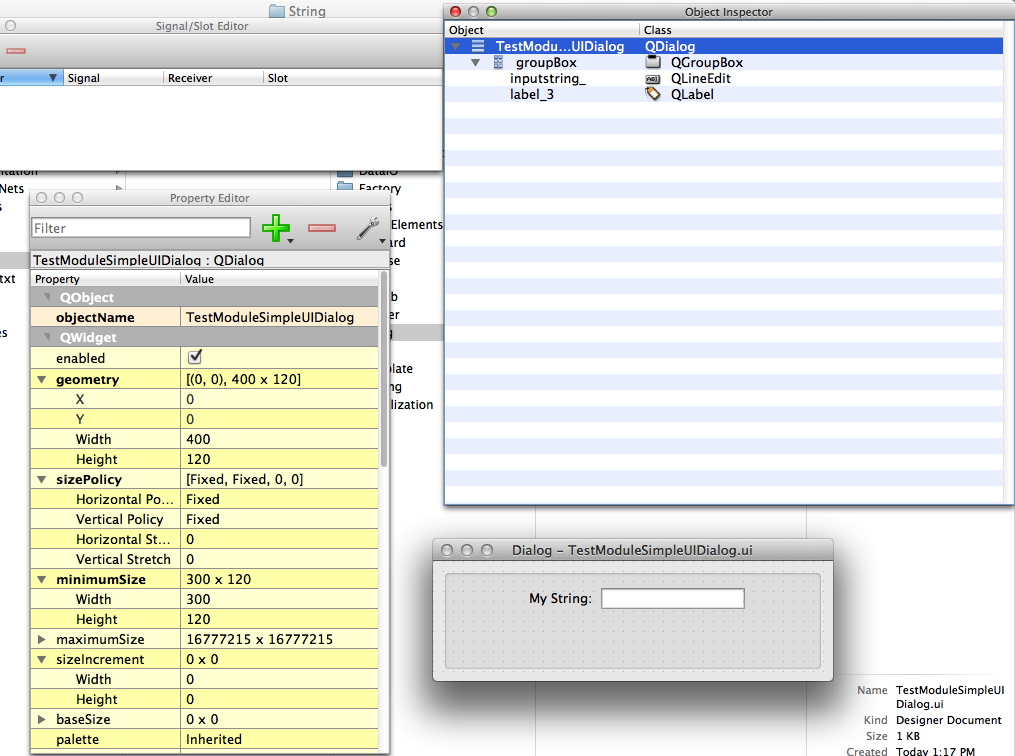
\includegraphics{SCIRun5ModuleGeneration_Figures/simpleUI.png}}
\caption{Module interface design file for the TestModuleSimpleUI module as seen in the Qt editor.}
\label{fig:simpleUI}
\end{figure}

Now that the module UI is designed, we need to link it to the module with the module dialog code.
Copy the \emph{ModuleDialog.cc} and the \emph{ModuleDialog.h} from the \emph{src/Interface/Modules/Template/} directory to the \emph{src/Interface/Modules/String/} directory, with the appropriate names (\emph{TestModuleSimpleUIDialog.cc} and \emph{TestModuleSimpleUIDialog.h}).
For the \emph{TestModuleSimpleUIDialog.h}, change the module name reference to the correct module name and delete the 'virtual void pull()' function.  The code should be very similar to the following:
\begin{verbatim}
#ifndef INTERFACE_MODULES_STRING_TestModuleSimpleUIDialog_H
#define INTERFACE_MODULES_STRING_TestModuleSimpleUIDialog_H

#include <Interface/Modules/String/ui_TestModuleSimpleUIDialog.h>
#include <Interface/Modules/Base/ModuleDialogGeneric.h>
#include <Interface/Modules/String/share.h>

namespace SCIRun {
namespace Gui {
  
class SCISHARE TestModuleSimpleUIDialog : public ModuleDialogGeneric,
  public Ui::TestModuleSimpleUIDialog
{
	Q_OBJECT
	
public:
  TestModuleSimpleUIDialog(const std::string& name,
    SCIRun::Dataflow::Networks::ModuleStateHandle state,
    QWidget* parent = 0);
};
}}
#endif
\end{verbatim}
The \emph{TestModuleSimpleUIDialog.cc} requires similar treatment, but will require the addition of few more changes.  Add and include for the module header file, change the namespace from 'Field' to 'StringManip', and delete the last two lines from the main function.
The code should be:
\begin{verbatim}
#include <Interface/Modules/String/TestModuleSimpleUIDialog.h>
#include <Modules/String/TestModuleSimpleUI.h>

using namespace SCIRun::Gui;
using namespace SCIRun::Dataflow::Networks;
using namespace SCIRun::Modules::StringManip;

TestModuleSimpleUIDialog::TestModuleSimpleUIDialog(const std::string& name, ModuleStateHandle state,
  QWidget* parent /* = 0 */)
  : ModuleDialogGeneric(state, parent)
{
  setupUi(this);
  setWindowTitle(QString::fromStdString(name));
  fixSize();
}
\end{verbatim}
This should be enough to create a UI for the TestModuleSimpleUI module, but it will not be able interact yet.
We will need to modify this file later to connect all the required inputs.  
For now, we can build SCIRun to test the UI design.  
Make sure that these three new files are added to the \emph{CMakeList.txt} in the \emph{src/Interface/Modules/String/} directory:
\begin{verbatim}

�

SET(Interface_Modules_String_FORMS
  
  ...
  
  TestModuleSimpleUIDialog.ui
)

SET(Interface_Modules_String_HEADERS

�

  TestModuleSimpleUIDialog.h
)

SET(Interface_Modules_String_SOURCES 
  
  ...
  
  TestModuleSimpleUIDialog.cc
)

�

\end{verbatim}

Once these files are added, SCIRun should build. 
Load SCIRun and place the TestModuleSimpleUI module.  
Open the UI for the module and make sure that looks correct.  


\section{Connecting UI to the Module}
\label{sec:connectUI}

Now we will work on connecting the input from the UI to the code in the module.  
Begin by modifying the \emph{TestModuleSimpleUIDialog.cc} to include a line that reads the input field and assigns it to a variable. 
This line needs to go near the end in the main function of the module dialog code
\begin{verbatim}
addLineEditManager(inputstring_,TestModuleSimpleUI::FormatString);
\end{verbatim}
This function will read the value of 'inputstring\_' and set it to 'FormatString', which we have included as if it was part of the 'TestModuleSimpleUI' namespace.  
We will need to include it as such, by adding it as a public function in the \emph{TestModuleSimpleUI.h} file.
\begin{verbatim}
static Core::Algorithms::AlgorithmParameterName FormatString;
\end{verbatim}
This should be the final declaration in the public list (after the 'staticInfo\_' declaration).
Another change in this file is to modify the 'setStateDefault' function so that it is not empty.  
Remove the curly brackets from this:
\begin{verbatim}
virtual void setStateDefaults() {};
\end{verbatim}
so that it is:
\begin{verbatim}
virtual void setStateDefaults();
\end{verbatim}
We need a couple more additions to make the value from the UI available for use in the main function code.  
In the \emph{TestModuleSimpleUI.cc} file, add the following line to the before the main execute function, i.e., right after declaring the namespaces.
\begin{verbatim}
SCIRun::Core::Algorithms::AlgorithmParameterName PrintStringIntoString::FormatString("FormatString");
\end{verbatim}

Next we need to be able to set the state defaults by creating context for the 'setStateDefault' function we just exposed.
Add this function just before the execute function.
\begin{verbatim}
void TestModuleSimpleUI::setStateDefaults()
{
  auto state = get_state();
  state->setValue(FormatString,std::string ("[Insert message here]"));
}
\end{verbatim}
With these three additions, the code should build.
If you load the module, you should she the default message ("[Insert message here]") in the input field.  
Changing this will still not affect the output because the execute function is still hard coded for a specific message.  

Now we need to change the execute function to use the UI inputs, which is very simple.  
Simply get the state of the module (\verb|auto state = get_state();|), then assign the output string variable to \verb|state -> getValue(FormatString).toString();| so that the function is as follows:
\begin{verbatim}
void
TestModuleSimpleUI::execute()
{
  std::string message_string;
  auto state = get_state();
  message_string = state -> getValue(FormatString).toString();
  StringHandle msH(new String(message_string));
  sendOutput(OutputString, msH);
}
\end{verbatim}
After building the software, you should now see that the output of module will be the same as the string that is put in the input field in the module UI.  

\section{Adding an Input Port}
\label{sec:addinput}

With the UI implemented and working, we will now add an optional input port to the module.  
This functionality is fairly simple in SCIRun5.  
We need to add the port in the \emph{TestModuleSimpleUI.h} file.  
First, replace the line:
\begin{verbatim}
public HasNoInputPorts,
\end{verbatim}
with:
\begin{verbatim}
public Has1InputPort<StringPortTag>,
\end{verbatim}
Next, we need to name the port in the list of public objects.  
Add:
\begin{verbatim}
INPUT_PORT(0, InputString, String);
\end{verbatim}
near the output port declaration.  
These changes are all that are needed in the header file, but we need to initialize the port in the .cc file.
In the \emph{TestModuleSimpleUI.cc}, add the initializing line to the module constructor function, which should be then:
\begin{verbatim}
TestModuleSimpleUI::TestModuleSimpleUI() : Module(staticInfo_)
{
  INITIALIZE_PORT(InputString);
  INITIALIZE_PORT(OutputString);
}
\end{verbatim}
These changes should allow the code to build with an input port, yet the input will not affect the output of the module. 

In the main execute function in \emph{TestModuleSimpleUI.cc}, we need to read whether there is an input, then use that input or the UI input if there is none.  
This is straight forward in SCIRun, the execute function will be:
\begin{verbatim}
void
TestModuleSimpleUI::execute()
{
  std::string message_string;
  auto  stringH = getOptionalInput(InputString);
  auto state = get_state();
  
  if (stringH && *stringH)
  {
    state -> setValue(FormatString, (*stringH) -> value());
  }
  
  message_string = state -> getValue(FormatString).toString();
  StringHandle msH(new String(message_string));
  sendOutput(OutputString, msH);
}
\end{verbatim}
This code reads an optional input, checks if it is not empty, and if so then changes the state variable to the input.  
By changing the state variable before assigning it to the output, it changes the UI input string also.  

This should be all the changes necessary to add inputs to this module.
Build SCIRun, then test the module using the CreateString and PrintDatatype modules.  
When there is no input, the value in the UI field is the output.  
When there is an output, the input port is the same as the output port, and the UI input field is set to the input string.  
This prevents the user from changing the input string while there is a string in the input port.  

For a slightly more complicated, yet much more useful module as an example, check out PrintStringIntoString.
The setup code is mostly the same, except there are dynamic ports, so much of the code will look very similar.  
 
\section{Finished Code}
\label{sec:finished}


%TODO add references to the files.  


%%%%%%%%%%%%%%%%%%%%%%%%%%%%%%%%%%%%%%%%%%%%%%%%%%%%%%%%%%%%%%%%%%%

\chapter{Example: Simple Module With Algorithm}

\begin{introduction}
%Scope: \hyperref[readdata]{Read Data File} - \hyperref[slice]{Slice} -
%\hyperref[visualize]{Visualize} - \hyperref[bbox]{Bounding Box} - \hyperref[isosurface]{Isosurface}
\end{introduction}


%TODO

%%%%%%%%%%%%%%%%%%%%%%%%%%%%%%%%%%%%%%%%%%%%%%%%%%%%%%%%%%%%%%%%%%%

\chapter{Converting Modules from SCIRun 4}

\begin{introduction}
Scope: \hyperref[sec:strategy]{Strategy} - \hyperref[sec:changes]{Common Function Changes} - \hyperref[sec:errors]{Common Build Errors}
\end{introduction}

\section{Strategy}
\label{sec:strategy}

\section{Common Function Changes}
\label{sec:changes}

\section{Common Build Errors}
\label{sec:errors}

%%%%%%%%%%%%%%%%%%%%%%%%%%%%%%%%%%%%%%%%%%%%%%%%%%%%%%%%%%%%%%%%%%%

\chapter{Creating Unit Tests}

\begin{introduction}
%Scope: \hyperref[readdata]{Read Data File} - \hyperref[slice]{Slice} -
%\hyperref[visualize]{Visualize} - \hyperref[bbox]{Bounding Box} - \hyperref[isosurface]{Isosurface}
\end{introduction}

You will at least need a testing network.  


%%%%%%%%%%%%%%%%%%%%%%%%%%%%%%%%%%%%%%%%%%%%%%%%%%%%%%%%%%%%%%%%%%%

\chapter{Documenting the New Module}

\begin{introduction}
%Scope: \hyperref[readdata]{Read Data File} - \hyperref[slice]{Slice} -
%\hyperref[visualize]{Visualize} - \hyperref[bbox]{Bounding Box} - \hyperref[isosurface]{Isosurface}
\end{introduction}

You should totally document the modules you add.  



%\begin{figure}[H]
%\scalebox{0.3}{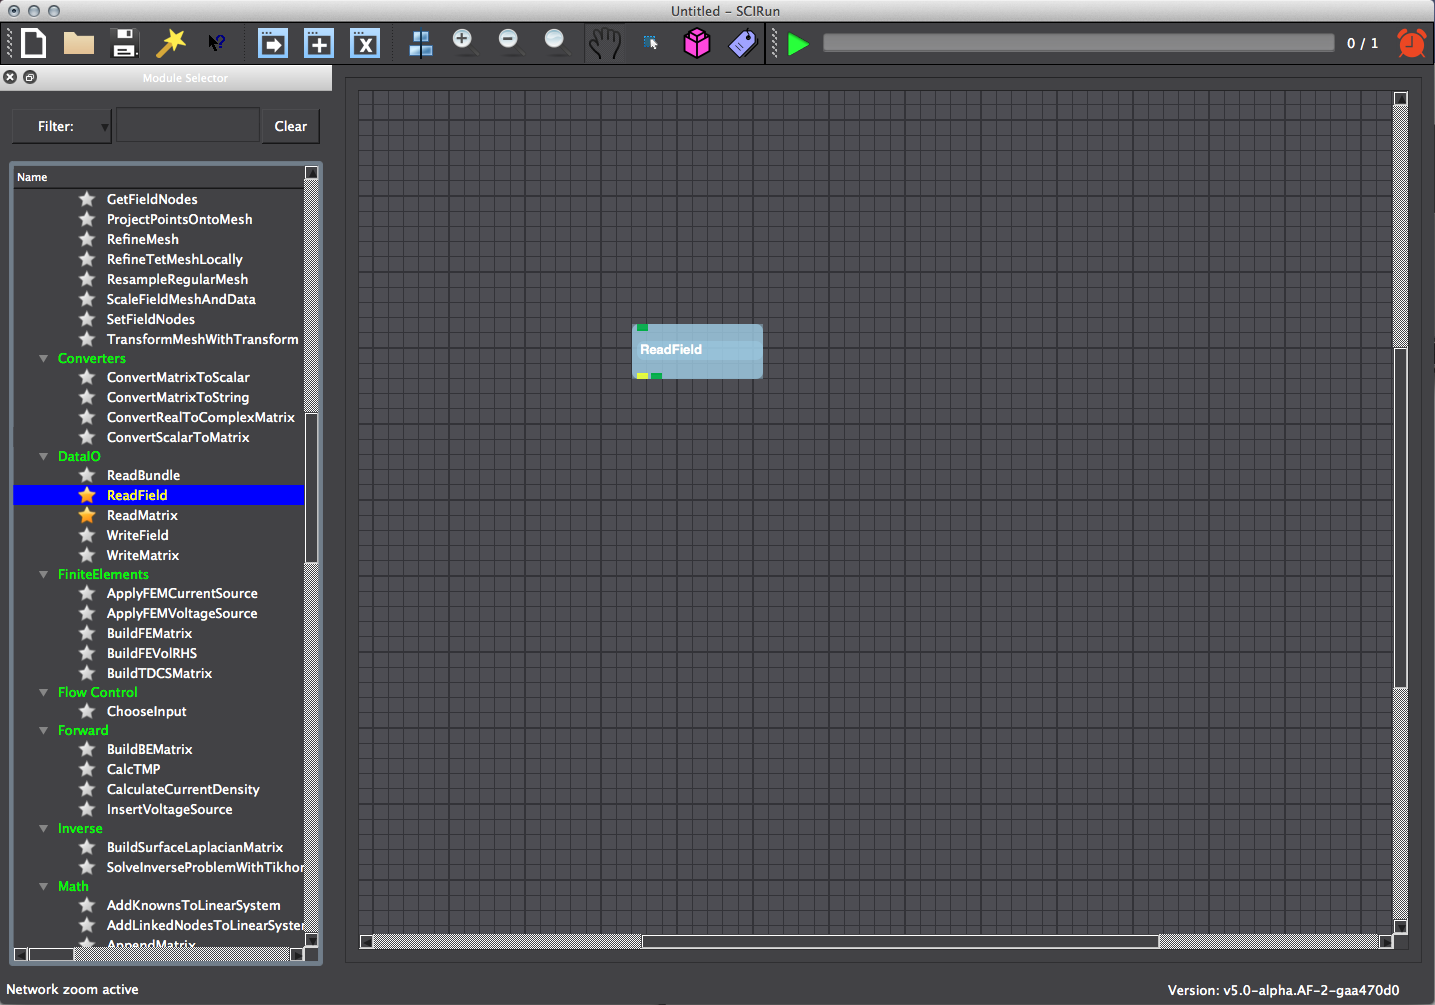
\includegraphics{BasicTutorial_figures/readfield.png}}
%\caption{Locate ReadField module.}
%\label{fig:readfield}
%\end{figure}


\end{document}
